\documentclass[a0]{a0poster}
% You might find the 'draft' option to a0 poster useful if you have
% lots of graphics, because they can take some time to process and
% display. (\documentclass[a0,draft]{a0poster})

%%
%% MATH DEFINITIONS   
%%

\def\({\left(}
\def\){\right)}

\def\inv#1{{\frac{1}{#1}}}
\def\ddt#1{\der{#1}{t}}
\def\ddx#1{\der{#1}{x}}
\def\ddz#1{\der{#1}{z}}
\def\der#1#2{{\frac{d#1}{d#2}}}
\def\derder#1#2{{d^2\frac{#1}{d{#2}^2}}}
\def\norm#1{\labs #1 \rabs}
\def\pder#1#2{{\frac{\partial#1}{\partial#2}}}
\def\pderder#1#2{{\frac{\partial^2#1}{\partial{#2}^2}}}
\def\pdt#1{\pder{#1}{t}}
\def\pdx#1{\pder{#1}{x}}
\def\pdxx#1{\pderder{#1}{x}}
\def\pdz#1{\pder{#1}{z}}
\def\pdzz#1{\pderder{#1}{z}}
\def\ssize#1{{\scriptsize #1}}

\def\bmat{\left[ \begin{array}}
\def\bna{\begin{array}}
\def\bneas{\begin{eqnarray*}}
\def\bnea{\begin{eqnarray}}
\def\bnes{\begin{displaymath}}
\def\bne{\begin{equation}}

\def\emat{\end{array} \right]}
\def\ena{\end{array}}
\def\eneas{\end{eqnarray*}}
\def\enea{\end{eqnarray}}
\def\enes{\end{displaymath}}
\def\ene{\end{equation}} 

\def\half{\frac{1}{2}} 

\def\revrxn#1#2{
\begin{array}{c} 
{#1}\\
\rightleftharpoons \\
{#2}
\end{array}
}

\def\Bold#1{\vspace{0.1in} \noindent {\bf \boldmath #1}}

\def\Sec#1{Section~\ref{#1}}
\def\Secs#1#2{Sections~\ref{#1}--\ref{#2}}
\def\SecsAnd#1#2{Sections~\ref{#1} and \ref{#2}}

\def\Eqn#1{Eq.~\ref{#1}}
\def\Eqns#1#2{Eqs.~\ref{#1}--\ref{#2}}
\def\EqnsAnd#1#2{Eqs.~\ref{#1} and \ref{#2}}

\def\Eq#1{Eq.~\ref{#1}}
\def\Eqs#1#2{Eqs.~\ref{#1}--\ref{#2}}
\def\EqsAnd#1#2{Eqs.~\ref{#1} and \ref{#2}}

\def\Fig#1{Fig.~\ref{#1}}
\def\Figs#1#2{Figs.~\ref{#1}--\ref{#2}}
\def\FigsAnd#1#2{Figs.~\ref{#1} and \ref{#2}}

\def\Figure#1{Figure~\ref{#1}}
\def\Figures#1#2{Figures~\ref{#1}--\ref{#2}}
\def\FiguresAnd#1#2{Figures~\ref{#1} and \ref{#2}}

\def\avg#1{\langle{#1}\rangle}
\def\Parens#1{\left({#1}\right)}

\def\Bold#1{{\bf #1}}
\def\Block#1#2{{\bf #1:} {#2}\\ }

\def\bfcite#1{{\bf\cite{#1}}}

\def\bpi{\boldsymbol \pi}
\def\E{\mathsf E}
\def\P{\mathsf P}
\def\Pr{\mathsf P}
\def\Var{\mathsf{Var}}


%%
%% CALCIUM DEFINITIONS   
%%

% My Definitions

\def\FcepsilonR1{Fc$\epsilon$R1}

\def\Ps{$\ps$}
\def\ps{{\rm s}^{-1}}

\def\Pms{$\pms$}
\def\pms{{\rm ms}^{-1}}

\def\UM{$\uM$}
\def\uM{\mu{\rm M}}

\def\Um{$\um$}
\def\um{\mu{\rm m}}

\def\Us{$\us$}
\def\us{\mu{\rm s}}

\def\Ums{$\ums$}
\def\ums{\mu{\rm m}^2}

\def\Nm{$\nm$}
\def\nm{\mu{\rm m}}

\def\Pumps{$\pumps$}
\def\pumps{\mu{\rm M}^{-1} {\rm s}^{-1}}

\def\Pumpms{$\pumpms$}
\def\pumpms{\mu{\rm M}^{-1} {\rm ms}^{-1}}

\def\UMps{$\uMps$}
\def\uMps{\mu{\rm M}/{\rm s}}

\def\Umpss{$\umpss$}
\def\umpss{\mu{\rm m}/{\rm s}^2}

\def\Umsps{$\umsps$}
\def\umsps{\mu{\rm m}^2/{\rm s}}

\def\Umspms{$\umspms$}
\def\umspms{\mu{\rm m}^2/{\rm ms}}

\def\Ryr{RyR}
\def\ip{{[{\rm IP}_3]}}

\def\Ip{${\rm IP}_3$}
\def\Ipr{${\rm IP}_3{\rm R}$}

\def\cad{[{\rm Ca}^{\rm 2+}]_{\rm d}}
\def\Cad{$\cad$}

\def\cabulk{[{\rm Ca}^{\rm 2+}]_{\rm bulk}}
\def\Cabulk{$\cabulk$}

\def\cainf{[{\rm Ca}^{\rm 2+}]_{\infty}}
\def\Cainf{$\cainf$}

\def\cai{[{\rm Ca}^{\rm 2+}]_{\rm i}}
\def\Cai{$\cai$}

\def\caext{[{\rm Ca}^{\rm 2+}]_{\rm ext}}
\def\Caext{$\caext$}

\def\cae{[{\rm Ca}^{\rm 2+}]_{\rm ER}}
\def\Cae{$\cae$}

\def\cat{[{\rm Ca}^{\rm 2+}]_{\rm T}}
\def\Cat{$\cat$}

\def\ve{{\varepsilon}}
\def\Bj{${\rm B}_j$}
\def\B{${\rm B}$}
\def\Bt{$\bt$}
\def\Ca{${\rm Ca}^{\rm 2+}$}
\def\K{${K}^{+}$}
\def\Cabj{${\rm CaB}_j$}
\def\Cab{${\rm CaB}$}
\def\Kj{$\kj$}
\def\Kjm{$\kjm$}
\def\Kjp{$\kjp$}
\def\Kmm{$\kmm$}
\def\Kkm{$\kkm$}
\def\Kmp{$\kmp$}
\def\Km{$\km$}
\def\Kp{$\kp$}
\def\bjt{\bj_T}
\def\b{[{\rm B}]}
\def\bj{[{\rm B}_j]}
\def\bmt{\bm_T}
\def\bt{\b_{\rm T}}
\def\bm{[B_m]}
\def\cabj{[{\rm CaB}_j]}
\def\cab{[{\rm CaB}]}
\def\ca{[{\rm Ca}^{2+}]}
\def\dc{D_c}
\def\dj{D_j}
\def\dm{D_m}
\def\db{D_b}
\def\kj{K_j}
\def\kjm{k^-_j}
\def\kjp{k^+_j}
\def\kmm{k^-_m}
\def\kmp{k^+_m}
\def\kkm{K_m}
\def\km{k^-}
\def\kp{k^+}

\def\wm{w^-}
\def\wp{w^+}
\def\minf{m_\infty}

% other ions

\def\mg{[{\rm Mg}^{2+}]}
\def\Mg{${\rm Mg}^{\rm 2+}$}





\def\Ca{Ca$^{2+}$}

\pagestyle{empty}
\setcounter{secnumdepth}{0}

% The textpos package is necessary to position textblocks at arbitary 
% places on the page.
\usepackage[absolute]{textpos}

% Graphics to include graphics. Times is nice on posters, but you
% might want to switch it off and go for CMR fonts.
\usepackage{graphics,wrapfig,times}


% These colours are tried and tested for titles and headers. Don't
% over use color!
\usepackage{color}
\definecolor{DarkBlue}{rgb}{0.1,0.1,0.5}
\definecolor{Red}{rgb}{0.9,0.0,0.1}
\definecolor{DarkGreen}{rgb}{0.1,0.4,0.1}

% Calcium defs
\def\Eq#1{Eq.~\ref{#1}}
\def\Eqs#1#2{Eqs.~\ref{#1}--\ref{#2}}
\def\EqsAnd#1#2{Eqs.~\ref{#1} and \ref{#2}}
\def\Figs#1{Figs.~\ref{#1}}
\def\bpi{\boldsymbol{\pi}} 
\def\E{\mathsf{E}} 
\def\Pr{\mathsf{P}} 
\def\Var{\mathsf{Var}} 
\def\Cov{\mathsf{Cov}} 
\def\be{\boldsymbol{e}} 
\def\beo{\boldsymbol{e}_\mathcal{O}}
\def\bec{\boldsymbol{e}_\mathcal{C}}
\def\io{I_\mathcal{O}}
\def\ic{I_\mathcal{C}}
\def\bu{\boldsymbol{u}} 
\def\bzero{\boldsymbol{0}} 
\def\bone{\boldsymbol{1}} 
\def\bx{\boldsymbol{x}} 
\def\by{\boldsymbol{y}} 
\def\bt{\boldsymbol{t}} 
\def\bk{\boldsymbol{k}} 
\def\bb{\boldsymbol{b}}
\def\diag{\mbox{diag}}
\def\c{\mathcal{C}}
\def\o{\mathcal{O}}
\def\r{\mathcal{R}}

\def\cT{c_{T}}
\def\cmyo{c_{myo}}
\def\csr{c_{sr}}
\def\cmyod{c_{myo}^d}
\def\csrd{c_{sr}^d}
\def\csrdn{ c_{sr}^{d,n}}
\def\csrdn{ c_{sr}^{d,n} }
\def\cmyodn{c_{myo}^{d ,\,n}}
\def\csrdn{c_{sr}^{d ,\,n}}
\def\cmyodstar{c_{myo}^{d,*}}
\def\csrdstar{c_{sr}^{d,*}}
\def\cmyoT{\hat {c}_{myo}}
\def\csrT{\hat{c}_{sr}}
\def\tildecmyod{{\tilde c}_{myo}^d }
\def\tildecsrd{{\tilde c}_{sr}^d }
\def\barcmyod{{\bar c}_{myo}^{\,d} }
\def\barcsrd{{\bar c}_{sr}^{\,d} }
\def\cmyodmin{c_{myo}^{d,min}}
\def\cmyodmax{c_{myo}^{d,max}}
\def\csrdmin{c_{sr}^{d,min}}
\def\csrdmax{c_{sr}^{d,max}}
\def\cext{c_{ext}}

\def\lambdasr{ \lambda_{sr} }
\def\lambdamyod{ \lambda_{myo}^{d} }
\def\lambdasrd{ \lambda_{sr}^{d} }
\def\lambdamyodT{ \Lambda_{myo}^{d} }
\def\lambdasrdT{ \Lambda_{sr}^{d} }

\def\pumsps{\mu\mathrm{M}^{-2}s^{-1}}
\def\Pumsps{$\pumsps$}

% see documentation for a0poster class for the size options here
\let\Textsize\normalsize
\def\Head#1{\noindent{\begin{center}\LARGE\color{DarkBlue} #1\end{center}}}
\def\LHead#1{\noindent{\LARGE\color{DarkGreen} #1}\medskip}
\def\Subhead#1{\noindent{\large\color{DarkGreen} #1}\medskip}
\def\Title#1{\noindent{\Huge\color{Red} #1}}

\TPGrid[40mm,40mm]{22}{12}      % 3 cols of width 7, plus 2 gaps width 1 OR 4 cols width 5 plus 3 gaps width 1

\parindent=0pt
\parskip=0.5\baselineskip

\usepackage{graphicx}
\usepackage{amssymb}
\usepackage{amsmath, amsthm}

\begin{document}



\begin{textblock}{19}(2.3,0)
\centering
\Title{\Huge Calcium Sparks and Homeostasis in a Minimal Model of Local and Global Calcium Responses in Quiescent Ventricular Myocytes}
\end{textblock}

\begin{textblock}{23}(0,.8)
\centering
\LHead{Jana~M.~Hartman$^{\rm{a}}$, Eric~A.~Sobie$^{\rm{b}}$, and Gregory~D.~Smith$^{\rm{a}}$\\}
\Subhead{
$^{a}$ Dept.\,of Applied Science, The College of William and Mary, Williamsburg, VA, 23187 \\
$^{b}$ Dept.\,of Pharm. \& Sys. Therapeutics, Mount Sinai School of Medicine, New York, NY  10029 \\
}
\end{textblock}

\begin{textblock}{1}(0.2,0)
\begin{figure}

\includegraphics[width=3.5in]{Figures/WMLogo}
\end{figure}
\end{textblock}

\begin{textblock}{23}(21.8,-0.2)
\begin{figure}

\includegraphics[height=2.1in]{Figures/MSLogo}
\end{figure}
\end{textblock}

%\begin{textblock}{7.4}(0,1.2)
%\begin{figure}
%\centering
%\includegraphics[width=12.0in]{Figures/ZimaTrim}
%\label{Zima}
%\end{figure}
%\end{textblock}

\begin{textblock}{7.4}(0,0.3)
\Head{--- Introduction ---}
We present a minimal whole cell model that accounts for both local and global aspects of \Ca\ signaling in quiescent ventricular myocytes.  We correlate our modeling results with recent experiments showing that tetracaine, an inhibitor of RyRs, causes a transient suppression of \Ca\ sparks followed by an increase in SR [\Ca], partial recovery of spark frequency, and an increase in \Ca\ spark duration [1]. 
\begin{figure}
\centering
\includegraphics[width=12.0in]{Figures/ZimaTrim2}
\label{Zima}
\end{figure}
\vspace{-0.5in}
\hspace{9in}{\small (Reproduced from Zima et al.~2008)}

\Head{--- Model Formulation ---}
\begin{wrapfigure}{r}{10.0in}
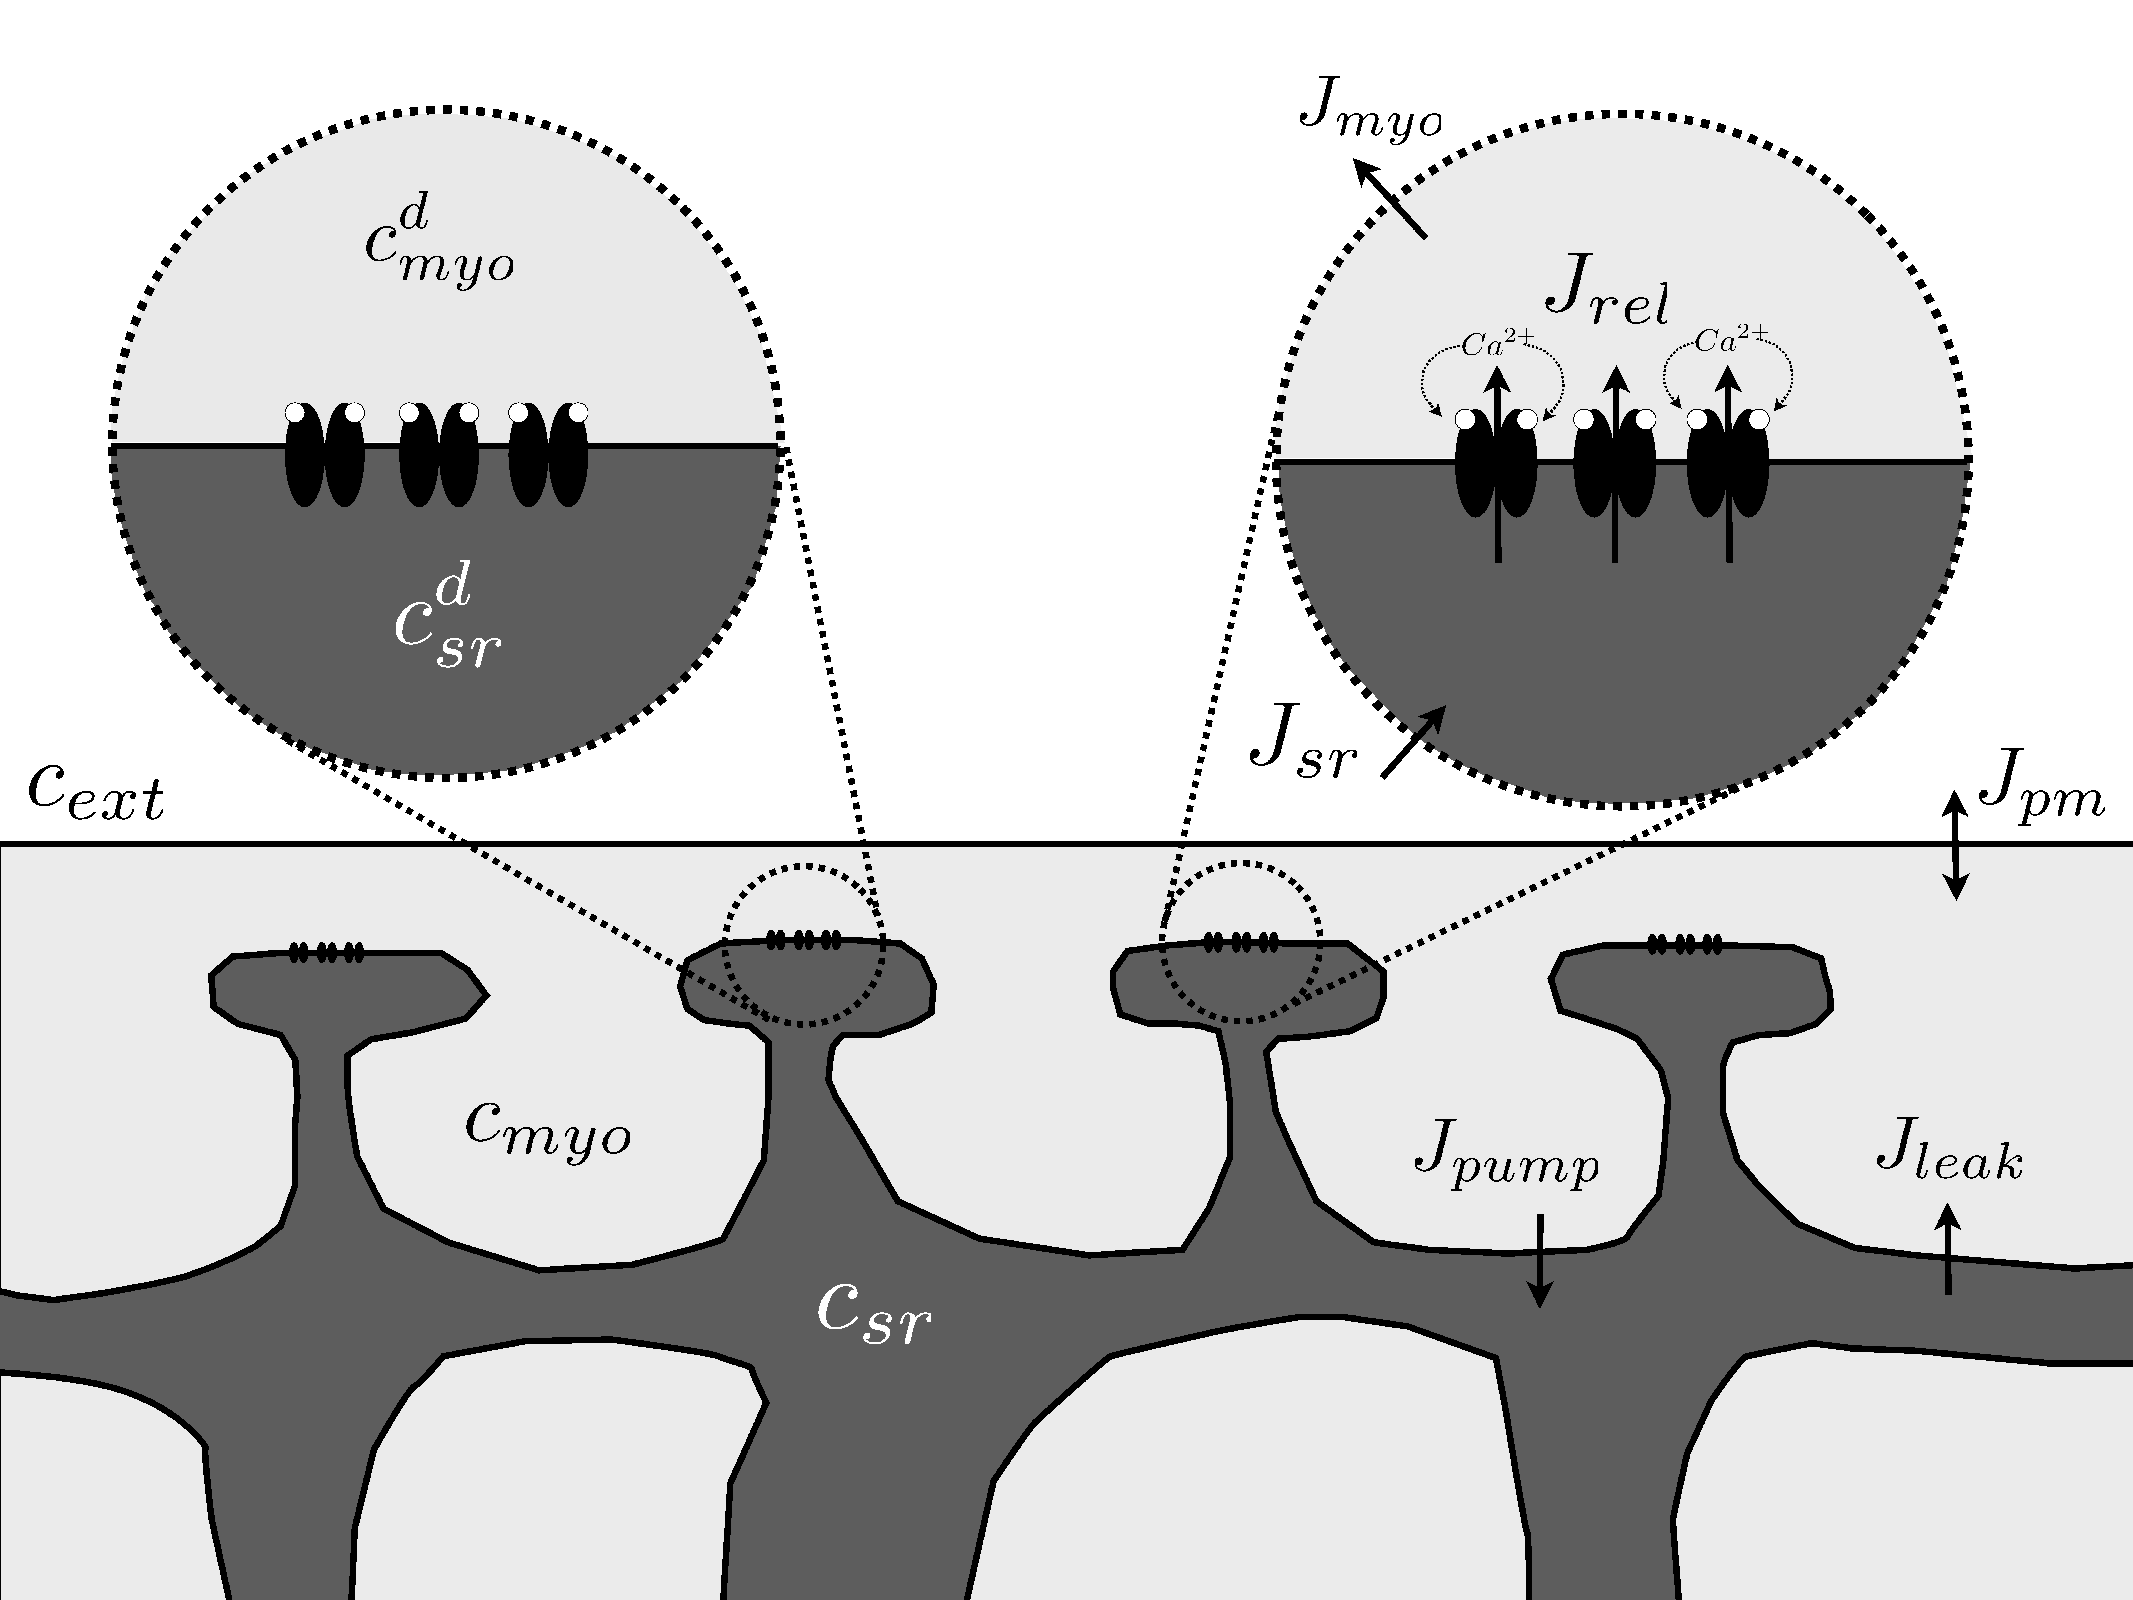
\includegraphics[width=9.0in]{Figures/ModelDiagram}
%\label{ModelDiagram}
\end{wrapfigure}
The model represents two bulk compartments: the SR ($c_{sr}$) and the myoplasm ($c_{myo}$).  The membrane of the SR contains multiple release sites, each of which includes a local \Ca\ domain on both sides of the membrane and is composed of N two-state RyRs with \Ca\ activation,
 \bne
 \large
 \begin{array}{ccc}
C & \revrxn{k_{co} (\cmyod)^2}{k_{oc}} & O \\
\end{array} 
\label{TWOSTATEDIAGRAM} 
\ene
By assuming mean-field coupling, the release site model becomes
\end{textblock}

\begin{textblock}{7.4}(0,7.5)
\bne
\label{NSTATETRANS}
\large
\begin{array}{ccccccccccc} 
  & N k_{co}(c_{myo}^{d ,\,0})^2 &   &    (N-1) k_{co}(c_{myo}^{d ,\,1})^2 &      &           2 k_{co} (c_{myo}^{d ,\,N-2})^2          &     & k_{co} (c_{myo}^{d ,\,N-1})^2 &  \\
0 & \rightleftharpoons & 1 &   \rightleftharpoons &   \ldots &   \rightleftharpoons& N-1 & \rightleftharpoons & N  \\
  & k_{oc}   &  & 2k_{oc}&    &(N-1) k_{oc}&  & N k_{oc} \\
\end{array} 
\ene

The fluxes shown in the above figure are given by
\end{textblock}

\begin{textblock}{3.5}(0,8.4)
\bne
\large
	J_{myo}^T = \sum_{n=0}^N f_n v_{myo}^T \left( \cmyodn - c_{myo} \right) 
\ene \bne
\large
	J_{sr}^T = \sum_{n=0}^N f_n v_{sr}^T \left( c_{sr} - \csrdn \right)
\ene
\end{textblock}

\begin{textblock}{7.4}(0,8.5)
 \bne
 \Large
	\hspace{6in} J_{pm} = k_{pm} \( \cext - \cmyo \)
\ene
\bne
 \Large
	\hspace{6in} J_{leak} = v_{leak} \left( \csr - \cmyo \right)
\ene
\bne
 \Large
	\hspace{6in} J_{pump} = \frac{v_{pump} \cmyo^2}{k_{pump}^2+\cmyo^2}. 
\ene

Under the assumption of a very large number of release sites, we may write whole cell model equations (see below) where 
$\lambdasr = V_{sr}/V_{myo}$, $V_{myo}$ and $V_{sr}$ are the effective myoplasmic and SR volumes (i.e., accounting 
for \Ca\ buffering capacity), $J_{myo}^{T}$ and $J_{sr}^T$ are total 
fluxes obtained by summing over all release sites,
 $Q = (q_{ij})$ is the infinitesimal generator matrix that corresponds to Eq.~\ref{NSTATETRANS}, and the elements of the row vector $\bpi(t)$ give the probability of finding a randomly sampled release site in each of $N+1$ possible states.
\bne
\Large
\der{\cmyo}{t} = J_{myo}^{T} + J_{leak} - J_{pump} + J_{pm}
\label{CCYT_ODE}
\ene
\bne
\Large
\der{\csr}{t} = \frac{1}{\lambdasr} \left( J_{sr}^T - J_{leak} + J_{pump}\right)
\label{CSR_ODE}
\ene
\bne
\Large
\quad\quad\quad \der{\bpi}{t}  = \bpi Q  \label{QMatrixForward}
\ene
\end{textblock}

\begin{textblock}{7.4}(0,12.0)

\includegraphics[width=6.0in]{Figures/CBLLogo}
\end{textblock}


%\begin{textblock}{1}(0.4,12.4)
%\begin{figure}
%
\includegraphics[width=3.0in]{Figures/CBLLogo}
%\end{figure}
%\end{textblock}

\begin{textblock}{7.4}(7.8,1.7)
\Head{--- Simulated Application of Tetracaine ---}
We simulate the application of tetracaine by decreasing the association rate constant $k_{co}$ in the single channel RyR model (Eq.~\ref{TWOSTATEDIAGRAM}).  The filled circles ($\bullet$) indicate the standard value ($k_{co} = 4.5$ ${\mu  \mathrm{M}}^{-2}s^{-1}$); the open circles ($\circ$) correspond to the simulated addition of tetracaine ($k_{co} = 0.5$ ${\mu  \mathrm{M}}^{-2}s^{-1}$).

\begin{figure}
\centering
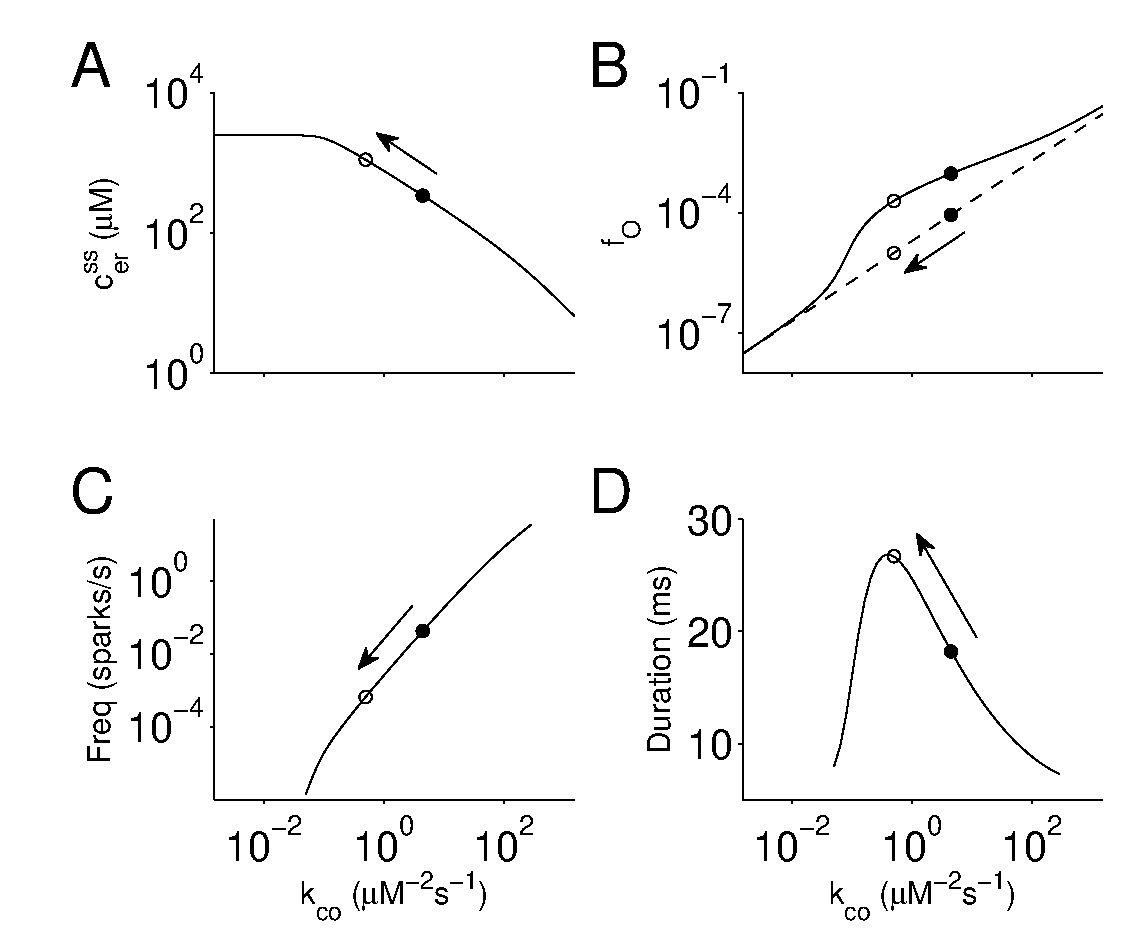
\includegraphics[width=13.0in]{Figures/Summary}
\label{Summary}
\end{figure}

\Head{--- Spark Frequency and Duration ---}
Below are representative \Ca\ sparks in the minimal whole cell model under three different steady-state conditions.  In order to confirm that the decreased spark frequency and increased mean spark duration are due to overloading of bulk SR [\Ca], the figure below (Control) shows a simulation with bulk SR [\Ca] ``clamped,'' RyR parameters that correspond to the addition of tetracaine and bulk SR [\Ca] that results from the standard parameters.  
\begin{figure}
\centering
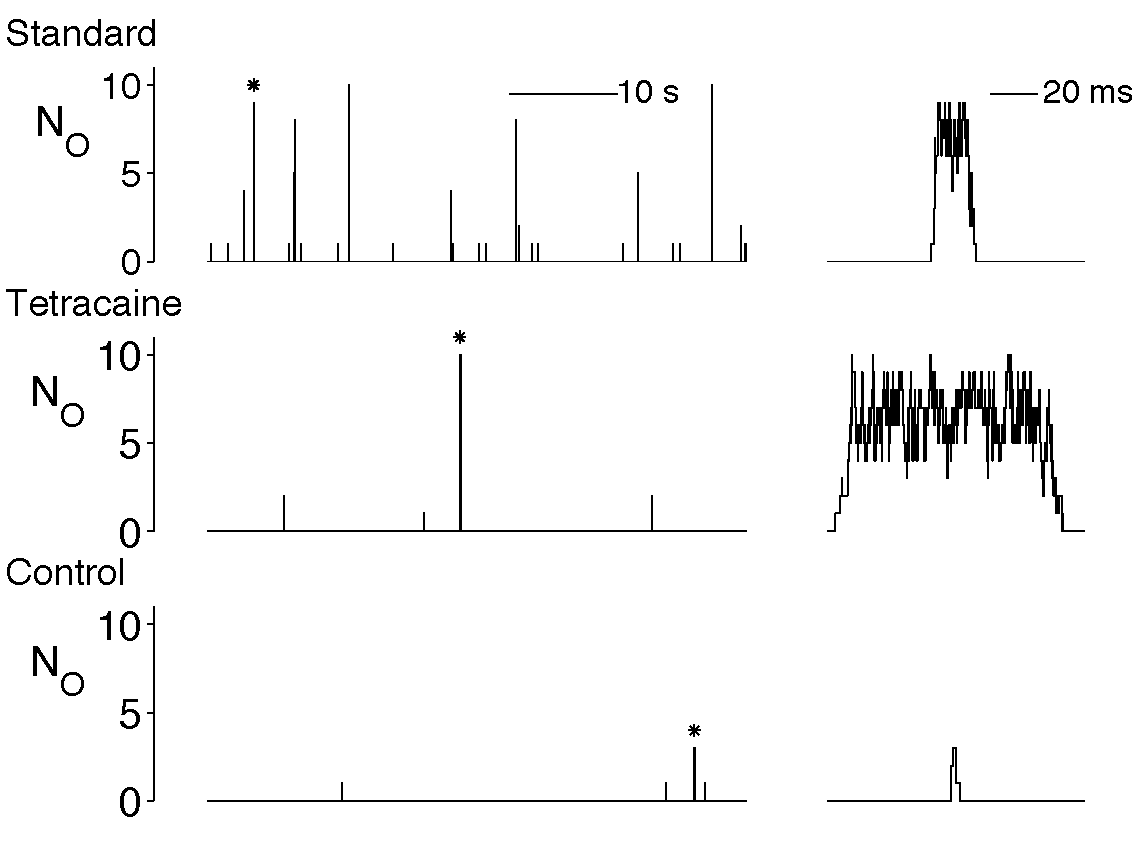
\includegraphics[width=12.0in]{Figures/SampleSparks}
\label{SampleSparks}
\end{figure}

\vspace{0.5in}
\begin{center}
\color{DarkGreen}
This material is based upon work supported by the National Science Foundation under Grant No.~0443843 and W\&M's Howard Hughes Medical Institute Undergraduate Biological Sciences Education Program.
\end{center}
\end{textblock}

\begin{textblock}{7.4}(15.6,0.3)
\Head{--- Aggregate Release Flux ---}
Because small amplitude events may not be detectable experimentally, it is of interest to dissect the aggregate release flux to determine the fraction of spontaneous release due to sparks vs.\ quarks. The following figure shows that tetracaine suppresses release mediated by sites with a small number of open channels more effectively than release mediated by sites with a large number of open channels.
\begin{figure}
\centering
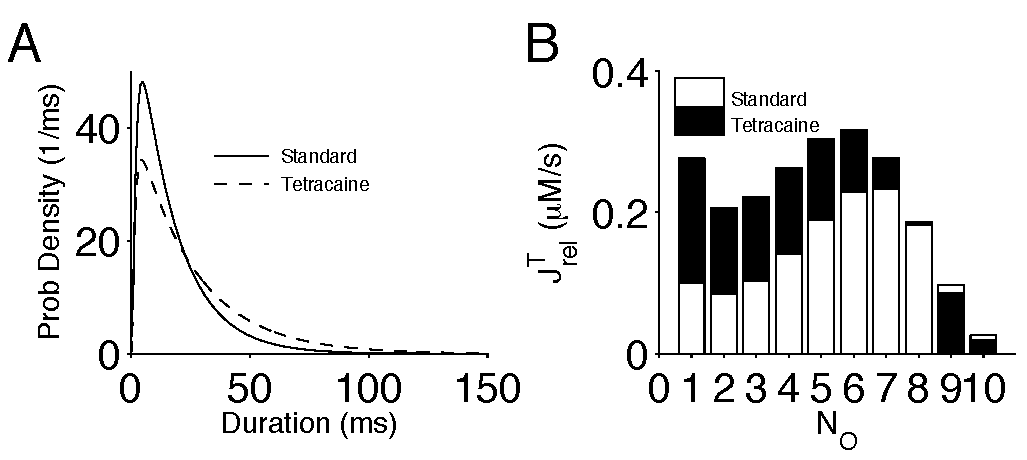
\includegraphics[width=13.0in]{Figures/DurDistJrel}
\label{DurDistJrel}
\end{figure}
\Head{--- Transient Effects of Tetracaine Application ---}
Consistent with experimental observations [1,2], the figure below shows that the initial application of tetracaine causes spark frequency to decrease, resulting in a slow increase in SR load that ultimately increases the mean spark duration.  Upon simulated washout of tetracaine there is a transient increase in spark frequency and a rapid depletion of SR [\Ca] from elevated to baseline values.
\begin{figure}
\centering
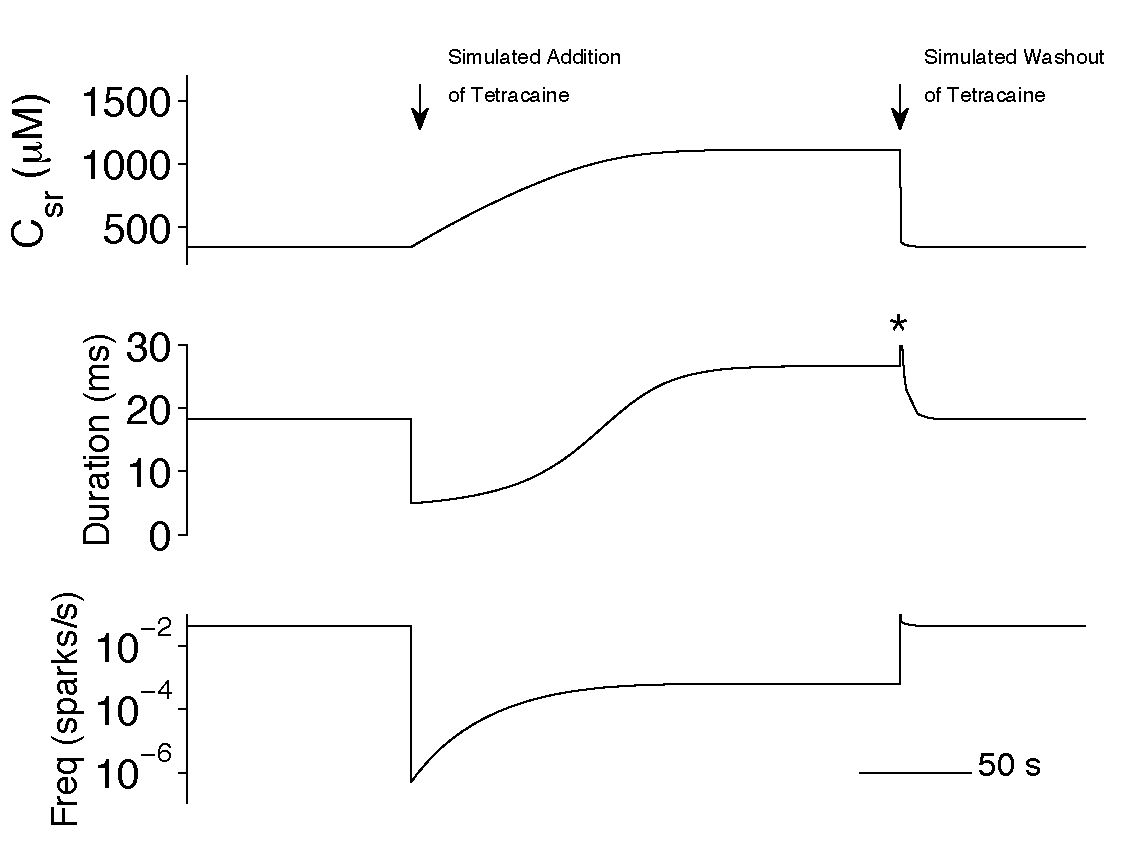
\includegraphics[width=10.0in]{Figures/Transients}
\label{Transients}
\end{figure}
\Head{--- RyR Inhibition Mechanism ---}
The open probability of the RyR can also be reduced by increasing the rate constant $k_{oc}$, analogous to the action of the pharmacological agent flecainide, which has been shown to reduce the dwell time in open states of the RyR [3].  When the same level of RyR inhibition is modeled as a decrease in open dwell time, the mean spark duration and frequency change, but other whole cell dynamics remain consistent.  
\begin{table}
\begin{center}
\begin{tabular}{|c|c|ccc|}
\hline
& standard & tetracaine & flecainide & dual mechanism \\
&  & ${\tau_C}{\uparrow}$ & ${\tau_O}{\downarrow}$ & ${\tau_C}{\uparrow}$ \& ${\tau_O} {\downarrow}$ \\
\hline
$k_{co}$ (${\mu  \mathrm{M}}^{-2}s^{-1}$) & $4.5$ & $0.5$ & $4.5$ & $1.5$ \\
$k_{oc}$ ($s^{-1}$) & $500$ & $500$ & $4500$ & $1500$ \\
\hline 
$f_O$ & $9.6 \times10^{-4}$ & $2.0 \times 10^{-4}$ & - & - \\
$score$ & 0.51 & 0.59 & - & - \\
$\csr$ ($\mu M$) & 342 & 1112 & - & - \\
duration (ms) & 18.2 & 26.7 & 2.97 & 8.90 \\
frequency (sparks/s) & 0.043 & $6.5 \times 10^{-4}$  & 0.053 & 0.0059 \\
\hline
\end{tabular}
\end{center}
\label{ParamsTwo}
\end{table}
\Head{--- References ---}

\small
1.  Zima, A., E. Picht, D. Bers, and L. Blatter. 2008. Partial inhibition of sarcoplasmic reticulum \Ca release evokes long-lasting \Ca release events in ventricular myocytes: Role of luminal \Ca in termination of \Ca release. \textit{Biophys. J.} 94:1867-79.

\begin{wrapfigure}{r}{2in}

\includegraphics[height=2in]{Figures/NSFLogo}
\end{wrapfigure}

2.  Gy{\"o}rke, S., V. Lukyanenko, and I. Gy{\"o}rke. 1997. Dual effects of tetracaine on spontaneous calcium release in rat ventricular myocytes. \textit{Journal of Physiology}. 500 Pt 2:297-309.

3.  Watanabe, H., N. Chopra, D. Laver, H. Hwang, S. Davies, D. Roach, H. Duff, D. Roden, A. Wilde, and B. Knollmann. 2009. Flecainide prevents catecholaminergic polymorphic ventricular tachycardia in mice and humans. \textit{Nature Medicine}. 15:380-383.

\end{textblock}





\end{document}
